%%%%%%%%%%%%%%%%%%%%%%%%%%%%%%%%%%%%%%%%%
% Academic Title Page
% LaTeX Template
% Version 2.0 (17/7/17)
%
% This template was downloaded from:
% http://www.LaTeXTemplates.com
%
% Original author:
% WikiBooks (LaTeX - Title Creation) with modifications by:
% Vel (vel@latextemplates.com)
%
% License:
% CC BY-NC-SA 3.0 (http://creativecommons.org/licenses/by-nc-sa/3.0/)
%%%%%%%%%%%%%%%%%%%%%%%%%%%%%%%%%%%%%%%%%

%----------------------------------------------------------------------------------------
%	PACKAGES AND OTHER DOCUMENT CONFIGURATIONS
%----------------------------------------------------------------------------------------

\documentclass[11pt]{article}

\usepackage{listings}
\usepackage{hyperref}
\usepackage{graphicx}
\usepackage{imakeidx}
\usepackage[utf8]{inputenc} % Required for inputting international characters
\usepackage[T1]{fontenc} % Output font encoding for international characters

\usepackage{mathpazo} % Palatino font

\usepackage{color}

\definecolor{dkgreen}{rgb}{0,0.6,0}
\definecolor{gray}{rgb}{0.5,0.5,0.5}
\definecolor{mauve}{rgb}{0.58,0,0.82}

\lstset{frame=tb,
  language=Python,
  aboveskip=3mm,
  belowskip=3mm,
  showstringspaces=false,
  columns=flexible,
  basicstyle={\small\ttfamily},
  numbers=none,
  numberstyle=\tiny\color{gray},
  keywordstyle=\color{blue},
  commentstyle=\color{dkgreen},
  stringstyle=\color{mauve},
  breaklines=true,
  breakatwhitespace=true,
  tabsize=3
}

\makeindex[columns=3, intoc]
\begin{document}

%----------------------------------------------------------------------------------------
%	TITLE PAGE
%----------------------------------------------------------------------------------------

\begin{titlepage} % Suppresses displaying the page number on the title page and the subsequent page counts as page 1
	\newcommand{\HRule}{\rule{\linewidth}{0.5mm}} % Defines a new command for horizontal lines, change thickness here
	
	\center % Centre everything on the page
	
	%------------------------------------------------
	%	Headings
	%------------------------------------------------
	
	\textsc{\LARGE AGH University of Science and Technology}\\[1.5cm] % Main heading such as the name of your university/college
	
	\textsc{\Large Cybersecurity: systems' and data protection}\\[0.5cm] % Major heading such as course name
	
	\textsc{\large Final report}\\[0.5cm] % Minor heading such as course title
	
	%------------------------------------------------
	%	Title
	%------------------------------------------------
	
	\HRule\\[0.4cm]
	
	{\huge\bfseries SYN flooding attack using Scapy}\\[0.4cm] % Title of your document
	
	\HRule\\[1.5cm]
	
	%------------------------------------------------
	%	Author(s)
	%------------------------------------------------
	
	{\large\textit{Author}}\\
	Beatriz \textsc{Galiana Carballido} % Your name
	
	%------------------------------------------------
	%	Date
	%------------------------------------------------
	
	\vfill\vfill\vfill % Position the date 3/4 down the remaining page
	
	{\large\today} % Date, change the \today to a set date if you want to be precise
	
	%------------------------------------------------
	%	Logo
	%------------------------------------------------
	
	\vfill\vfill
	
\includegraphics[width=0.2\textwidth]{agh-logo.png}\\[1cm] % Include a department/university logo - this will require the graphicx package
	 
	%----------------------------------------------------------------------------------------
	
	\vfill % Push the date up 1/4 of the remaining page
	
\end{titlepage}


\tableofcontents
\clearpage

%----------------------------------------------------------------------------------------

\section{Introduction to DoS attacks and TCP/IP connections}
Servers have become the target to many attacks. Some of these try to stop, temporarily or indefinitely, legitimate clients from accessing to the resources provided by the server, these kind of attacks are known as denial of service attacks (DoS). Denial of service may be indistinguishable from a heavy, but legitimate, load on the network: users might have difficulties connecting to the web site simply because too many people are trying to connect simutaneously.\vspace{5mm}

The Transmission Control Protocol (TCP) is one of the main protocols of the Internet protocol suite. It complemented the Internet Protocol (IP) in the initial network implementation so that is why the entire suite is commonly referred to as TCP/IP. TCP operates at a higher level than IP (which takes care of lower-level transmissions from host to host using the IP addresses). TCP provides reliable, ordered, and error-checked delivery of a stream of bytes between applications running on hosts that are communicating using an IP network.\vspace{5mm}

For a TCP connection to be established this three-way handshake needs to be performed between the client and the server. The client system begins the handshake by sending a SYN message to the server. The server then acknowledges the SYN message by sending SYN-ACK message to the client. The client then finishes establishing the connection by responding with an ACK message. The connection between the client and the server is then open, and data can be exchanged between them.\vspace{5mm}

The SYN flooding attack is based in the way the three-way handshake that begins a TCP connection works.

\begin{center}
\vfill\vfill
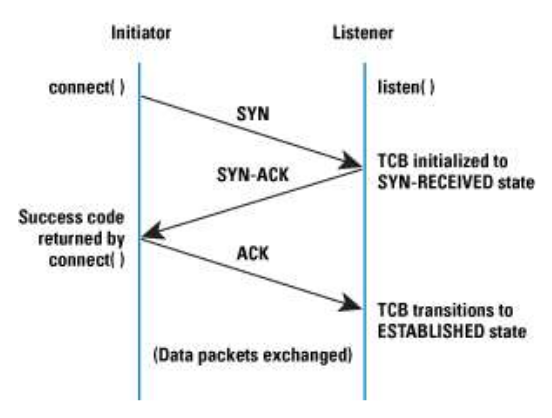
\includegraphics[width=0.5\textwidth]{3wayhandshake.png}\\[1cm]
\end{center}

\section{SYN Flood attack}
A SYN flood attack is a form of denial of service attack in which the attacker, by taking advantage of the TCP three-way handshake, sends a succession of SYN requests to a target server attempting to consume enough resources in order to make it unavailable for answering other legitimate petitions.\vspace{5mm}

The attack starts when the client sends a SYN packet to open the connection. Then the target server will reply with an SYN-ACK and waits for the ACK of the client to establish the connection. This ACK will never come: the attacker can either simply not respond with the expected ACK or it could have sent an spoofed IP address that corresponds to a client that does not exist (ergo will never answer with the ACK packet). This will create a number of half-open connections on the target server as the connection is kept open, in a “SYN\_RECV” state, which will eventually consume the target server's resources.\vspace{5mm}

The aim of this report is to explain the technical details as well as the procedure followed in order to perform a SYN flood attack implemented with Python and Scapy using VirtualBox machines.\vspace{5mm}

Here is a view of the message flow during a TCP 3-way handshake while performing a SYN flood attack:

\begin{center}
\vfill
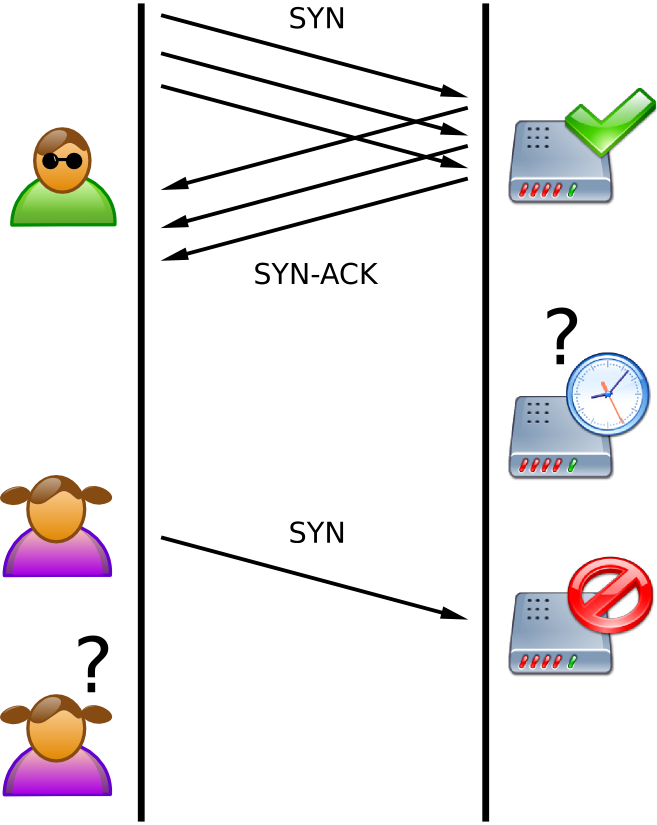
\includegraphics[width=0.4\textwidth]{tcp-synflood.png}\\[1cm]
\end{center}

\clearpage

\section{Why using Scapy}
\href{https://scapy.net}{Scapy} is a powerful interactive packet manipulation tool written in Python that allows us to end, sniff and dissect network packets. It is able to forge or decode packets of a wide number of protocols, send them on the wire, capture them, match requests and replies, among other things. It can easily handle most classical tasks like scanning, tracerouting, probing, unit tests, attacks or network discovery.\vspace{5mm}

\textbf{What's special about Scapy?} It does not interpret, it decodes.\vspace{5mm}

Machines are good at decoding and can sometimes help humans with that. Interpretation is reserved for human beings. Some programs try to mimic this behavior. For instance they say “this port is open” instead of “I received a SYN-ACK”. Sometimes they are right. Sometimes they are not. It might be easier for beginners, but when you know what you’re doing, you keep on trying to deduce what really happened from the program’s interpretation to make your own, which is hard because you lost a big amount of information.\vspace{5mm}

Moreover, with most other networking tools, you won’t build something the author did not imagine. These tools have been built for a specific goal and can’t deviate much from it. Scapy tries to overcome those problems. It enables you to build exactly the packets you want. You’re free to put any value you want in any field you want and stack them like you want. You’re the adult after all.\vspace{5mm}

In this report, we will be taking advantage of that freedom Scapy offers to craft malformed packets that will be sent to the target server. Since it is written in Python, we will write really simple Python scripts using Scapy as a library to achieve that.
\clearpage

\section{Implementation details of the attack}
In order to perform the attack, we will create a Python script which will generate several SYN packets using Scapy. This script will be executed in two VirtualBox machines that will be attackers and will be sent to another VM that will work as our target server.\vspace{5mm}

\subsection{\textbf{\texttt{\ttfamily{iptables}}} rules}
\texttt{\ttfamily{iptables}} is a Linux native firewall which comes pre-installed with most distributions. It is the userspace command line program used to configure the Linux 2.4.x and later packet filtering ruleset. It is usually targeted towards system administrators.\vspace{5mm}

For the attack to be successful we also need to modify an \texttt{\ttfamily{iptables}} rule that will only apply to the kernel, so it will not interfere with our Scapy application (as this happens in the application layer). This rule will drop all packages that have RST flag. The reason this needs to be done is because the kernel will send RST responses (resets) to the target when it sees the packets that are being sent with Scapy, since the kernel didn’t initiate this TCP communication. Using this iptables rule, the kernel’s RSTs will not get to the target.\vspace{5mm}

The following rule must be introduce on the attacker machines:\vspace{5mm}

\texttt{\ttfamily{iptables –A OUTPUT –p tcp –s <machine's IP address> --tcp-flags RST RST –j DROP}}\vspace{5mm}

\subsection{Virtual machines' deployment}
As it has been mentioned before, we will create three virtual machines using VirtualBox, two of them will be attackers and the other will perform the victim's role. They will run Ubuntu Server 18.04.3 and the victim will have an apache server running on port 80.\vspace{5mm}

The machines will be connected through the VirtualBox “Hostonly” network adapter. By using this method, VirtualBox creates virtual adapters for connections and doesn't try to use a physical network adapter. This setup requires creating a host-only adapter (if none exists).

\subsection{Description of the SYN flooding script}
This script is based on the original created by \href{https://github.com/subodhp}{Subodh Pachghare} in which the VM attacker sends malformed SYN connection packets to the target:\vspace{5mm}

\begin{lstlisting}

#! /usr/bin/env python
import sys
from scapy.all import *
print("Field Values of malformed packet sent")
# Create malformed packet
p = IP(dst = sys.argv[1], id = 1111, ttl = 99)/TCP(sport = RandShort(), dport=80, seq = 12345, ack = 1000, window = 1000, flags = "S")
ls(p)
print("Sending Packets in 0.3 second intervals for timeout of 4 sec")
ans, unans = srloop(p, inter = 0.3, retry = 2, timeout=4)
print("Summary of answered packets")
ans.summary()
print("---------------------------")
print("Summary of unanswered packets")
unans.summary()
print("source port flags in response")
for s,r in ans:
    print r.sprintf("%TCP.sport% \t %TCP.flags%")

\end{lstlisting}

\vspace{5mm}

Let's take a look at some of the details of the malformed packet: the destination address of the packet is passed as a parameter, it will be the address of the victim server (virtual machine). The source port is randomly generated using the \texttt{\ttfamily{RandShort()}} function. Lastly, the TCP flags are set to "S", in order to send a SYN packet.\vspace{5mm}

We will also use the method \texttt{\ttfamily{srloop()}} which sends a packet and continues to resend it after each response is received. This method returns a tuple of answered and unanswered packets, we will print a summary of those packets, too, so we can see the response of the target server.\vspace{5mm}

To end, printing the flag of the response packets allows us to check that the target replies are SYN-ACK (SA) responses.\vspace{5mm}

This SA shows that the server “thinks” the ACK from attacker was lost, so it keeps re-sending it. The connection on the target server remains in the SYN\_RECV state for 3 minutes for each port, as per the \texttt{\ttfamily{\href{https://sysctl-explorer.net/net/ipv4/tcp\_synack\_retries/}{net.ipv4.tcp\_synack\_retries}}} parameter, whose default value is set to 5 in Linux. After these retries, the kernel closes the connection.\vspace{5mm}

\section{Demo}
This demo shows the attacked being performed as it has been described in the prior section.

\section{Conclusion}
In this report we have approached some of the definitions related to concepts used in a SYN flood attack using Scapy and understood how a Python script to perform said attack works. The conclusions drawn are that this attack is one of most common DoS attacks due to the availabily of the tools that are required. A single security component is unable to properly defend a network which is why many security components must work together to defend a victim. For further reading, there are some proposed methods that can be found in the paper \emph{\href{http://citeseerx.ist.psu.edu/viewdoc/download?doi=10.1.1.206.5378&rep=rep1&type=pdf}{Three Counter Defense Mechanism for TCP SYN Flooding Attacks}}. 

\section{References and bibliography}

The scripts shown in this report as well as the .tex document used for composed the report can be found at the GitHub repository linked \href{https://github.com/beagaliana/syn-flooding-attack}{here}.\vspace{5mm}

\url{https://www.owasp.org/index.php/Denial\_of\_Service}\break
\url{https://resources.sei.cmu.edu/asset\_files/WhitePaper/1996\_019\_001\_496172.pdf#page=123}\break
\url{http://citeseerx.ist.psu.edu/viewdoc/download?doi=10.1.1.206.5378&rep=rep1&type=pdf}\break
\url{https://en.wikipedia.org/wiki/SYN\_flood}\break
\url{https://scapy.readthedocs.io/en/latest/introduction.html#about-scapy}\break
\url{https://www.virtualbox.org/manual/ch06.html#network\_hostonly}\break
\url{https://condor.depaul.edu/glancast/443class/docs/vbox\_host-only\_setup.html}\break
\url{https://kerneltalks.com/networking/basics-of-iptables-linux-firewall/}\break
\url{https://www.netfilter.org/projects/iptables/index.html}\break
\url{https://thepacketgeek.com/scapy-p-06-sending-and-receiving-with-scapy/}\break
\url{https://sysctl-explorer.net/net/ipv4/tcp\_synack\_retries/}\break

%----------------------------------------------------------------------------------------
\printindex
\end{document}
